\section{Introduction}
In this project, we simulate an indoor localization/tracking system through a wireless sensor network (WSN).
The sensor acquire the received signal strength (RSS) on a signal broadcast by a target to be located.

\subsection{Aims of the project}

\begin{enumerate}
    \item Simulation of a localization/tracking problem in WSNs
    \item Implementation of a localization/tracking distributed algorithm
    \item Analysis of the results
\end{enumerate}

\subsection{Physical setting}

\begin{itemize}
    \item Environment: square room of \SI{100}{\metre\squared}
    \item Grid: $p = 100$ square cells of \SI{1}{\metre\squared}
    \item Reference points: centers of the cells
    \item RSS model: indoor empirical model defined by the IEEE 802.15.4 standard
        \begin{equation}
            RSS(d) = \begin{cases}
                P_t - 40.2 - 20\log{d} + \eta & , \text{if $d\leq \SI{8}{\metre}$}\\
                P_t - 58.5 - 33\log{d} + \eta & , \text{if $d > \SI{8}{\metre}$}
            \end{cases}
        \end{equation}
        where $P_t=25$, $\eta$ is a Gaussian noise $\eta \sim \mathcal{N}(0,\sigma^2)$, $\sigma = 0.5$.
\end{itemize}

\subsection{WSN}

\begin{itemize}
    \item $n = 25$ sensors
    \item Deployment:
    \begin{itemize}
        \item \emph{uniformly} at random positions; each sensor is connected with sensors at distance $\le r$.
        \item \emph{grid} topology: the sensors are deployed on a grid $5 \times 5$; sensors are connected to 
        4 closest sensors (3 or 2 on the boundaries)
    \end{itemize}
\end{itemize}

\subsection{Data preprocessing}

To generate the data for the execution of the project, the script \highlight{build\_data.m} must be executed first.
It generates the file \highlight{data\_cps.m} which stores all the data used by the other scripts. The user can choose
whether to generate a random topology for the sensor network or a grid mesh. For completeness, we analyzed both the
situations.

\begin{figure}
    \begin{subfigure}{0.45\textwidth}
        \centering
        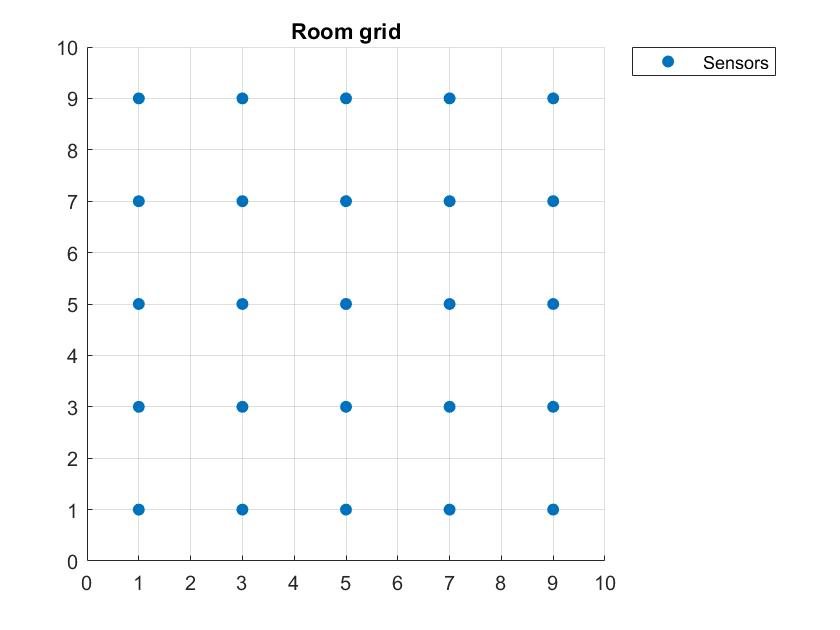
\includegraphics[width=\textwidth]{img/room_grid.jpg}
        \caption{Grid topology}
    \end{subfigure}
    \hfill
    \begin{subfigure}{0.45\textwidth}
        \centering
        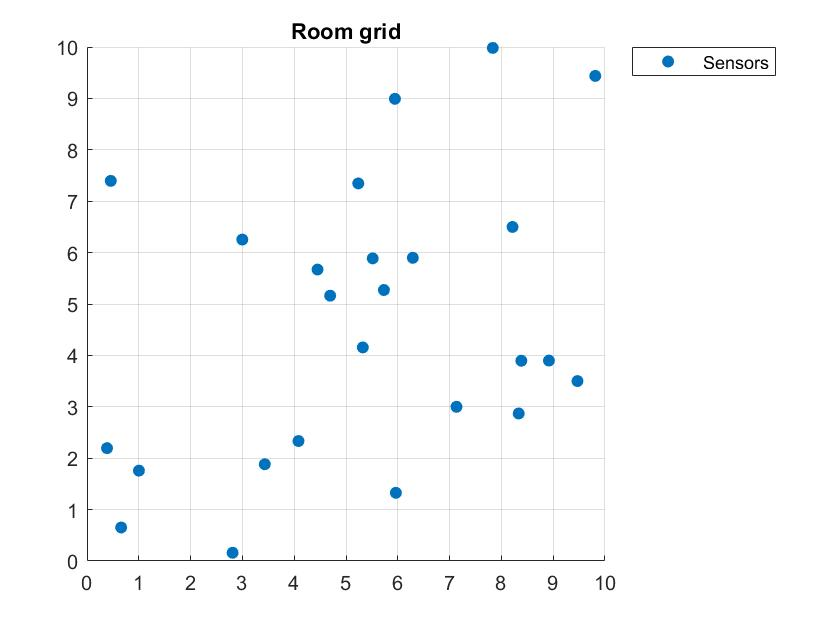
\includegraphics[width=\textwidth]{img/room_uniform.jpg}
        \caption{Uniform topology}
    \end{subfigure}
    \caption{Room topology}
\end{figure}